\section{Einleitung} % (fold)
\label{sec:einleitung}
	In diesem Versuch wird die experimentelle Umsetzung des Fourierschen Theorems untersucht.
	
\section{Theorie} % (fold)
\label{sec:theorie}
	\subsection{Das Fouriersche Theorem und Fourieranalyse}
	\label{subsec:fourier}

		In der Physik spielen periodische Vorg"ange eine zentrale Rolle.
		Sie lassen sich in bestimmten F"allen gut durch einfache $\sin$- oder $\cos$-Funktionene beschreiben, ben"otigen meist jedoch eine komplexere Beschreibung.

		Das Fouriersche Theorem besagt, dass jede periodische Funktion mit der Periodendauer $T$ durch die folgende Unendliche Reihe von $\sin$- und $\cos$-Funktionen dargestellt werden kann, wenn diese konvergiert:

		\begin{equation}
			f(t) = \frac{1}{2}a_0 + \sum_{\mathrm{n}=1}^\infty \left(a_\mathrm{n} \cos{\left(n \omega t\right)} + b_\mathrm{n} \sin{\left(n \omega t\right)}\right) \,. \label{eqn:fourier}
		\end{equation}

		F"ur die Kreisfrequenz $\omega$ und die Koeffizienten $a_\mathrm{n}$ und $b_\mathrm{n}$ mit $n \in \mathbb{N}_{\geq 1}$ gilt dabei:

		\begin{eqnarray}
			\nonumber \omega & = & \frac{2 \pi}{T} \,, \\
			\label{eqn:a_n} a_\mathrm{n} & = & \frac{2}{T} \int_0^T{f(t) \cos{\left(n \omega t\right)} \mathrm{d}t} \,, \\
			\label{eqn:b_n} b_\mathrm{n} & = & \frac{2}{T} \int_0^T{f(t) \sin{\left(n \omega t\right)} \mathrm{d}t} \,, \\
			\nonumber \frac{a_0}{2} & = & \frac{1}{T} \int_0^T{f(t) \mathrm{d}t} \,.
		\end{eqnarray}

		Die Koeffizienten m"ussen dabei f"ur gro"se n gegen 0 streben, damit die Fourierriehe konvergiert.
		Falls die Funktion $f$ zudem an einer Stelle $t_0$ unstetig ist, besitzt die Fourierriehe an dieser Stelle eine endliche Abweichung zu $f$.
		Dies wird als Gibbsches Ph"anomen bezeichnet.

		\begin{wrapfigure}{r}{6cm}
			\centering
			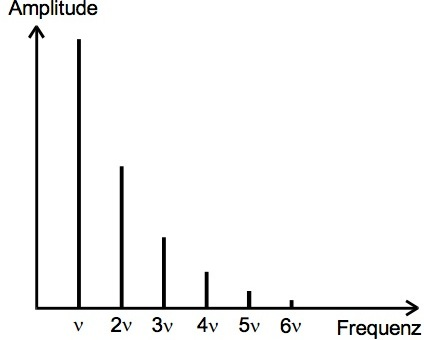
\includegraphics[width = 5cm]{img/spektrum.jpeg}
			\captionsetup{format=plain}
			\caption{Frequenzspektrum einer Funktion \cite{anleitung}.}
			\label{fig:spektrum}
		\end{wrapfigure}

		Die Ermittlung der Fourierkoeffizienten bezeichnet man als Fourieranalyse.
		Bei geraden Funktionen verschwinden dabei alle $b_\mathrm{n}$-, bei ungeraden verschwinden alle $a_\mathrm{n}$-Anteile.

		Als Spektrum bezeichnet man zudem das Bild aller Amplituden $a_\mathrm{n}$ und $b_\mathrm{n}$, aufgetragen gegen die Frequenz $\nu$.
		Abbildung \ref{fig:spektrum} zeigt beispielsweise ein Linienspektrum.

		\clearpage

	\subsection{Fouriertransformation}
	\label{subsec:trafo}
		Als Fouriertransformation bezeichnet man die Bestimmung des gesamten Frequenzspektrums einer Funktion $f$.
		Im Gegensatz zur Fourieranalyse ist es dabei egal, ob $f$ periodisch oder nichtperiodisch ist.
		Eine periodische Funktion f"uhrt lediglich auf das in Kapitel \ref{subsec:fourier} beschriebene Frequenzspektrum mit diskreten Amplituden (den Koeffizienten $a_\mathrm{n}$ und $b_\mathrm{n}$), w"ahrend eine nichtperiodische Funktion ein kontinuierliches Spektrum $g(\nu)$ liefert.
		Zudem l"asst sich mit Kenntnis des Frequenzspektrums, durch R"ucktransformation von $g$, die Funktion selbst finden:

		\begin{eqnarray}
			\label{eqn:trafo} g(\nu) & = & \int_{-\infty}^\infty{f(t) e^{i\nu t} \mathrm{d}t} \\
			\label{eqn:ruecktrafo} \Leftrightarrow \quad f(t) & = & \frac{1}{2 \pi} \int_{-\infty}^{\infty}{g(\nu) e^{-i\nu t} \mathrm{d}\nu} \,.
		\end{eqnarray}

		Da es praktisch unm"oglich ist, in Gleichung \eqref{eqn:trafo} "uber den unendlichen Zeitraum zu integrieren, treten bei der Umsetzung Fehler auf und die Periodizit"at von f geht verloren.
		Statt diskreten Frequenzen liefert die Transformation eine stetige Funktion mit Linien endlicher Breite.